%%%%%%%%%%%%%%%%%%%%%%%%%%%%%%%%%%%%%%%%%
% Journal Article
% LaTeX Template
% Version 1.3 (9/9/13)
%
% This template has been downloaded from:
% http://www.LaTeXTemplates.com
%
% Original author:
% Frits Wenneker (http://www.howtotex.com)
%
% License:
% CC BY-NC-SA 3.0 (http://creativecommons.org/licenses/by-nc-sa/3.0/)
%
%%%%%%%%%%%%%%%%%%%%%%%%%%%%%%%%%%%%%%%%%

%----------------------------------------------------------------------------------------
%	PACKAGES AND OTHER DOCUMENT CONFIGURATIONS
%----------------------------------------------------------------------------------------

\documentclass[twoside]{article}

\usepackage{lipsum} % Package to generate dummy text throughout this template
%\usepackage[caption=false]{subfig}
%\captionsetup[subfigure]{labelformat=brace}
\usepackage{graphicx, bm} % Required to insert images
\usepackage[]{algorithm2e}
\usepackage{capt-of}%%To get the caption
\usepackage{listings} % Required for insertion of code
\usepackage[usenames,dvipsnames]{color} % Required for custom colors
\usepackage[sc]{mathpazo} % Use the Palatino font
\usepackage[T1]{fontenc} % Use 8-bit encoding that has 256 glyphs
\linespread{1.05} % Line spacing - Palatino needs more space between lines
\usepackage{microtype} % Slightly tweak font spacing for aesthetics

\usepackage{amsmath}
\usepackage{amssymb}

\usepackage[hmarginratio=1:1,top=32mm,columnsep=20pt]{geometry} % Document margins
\usepackage{multicol} % Used for the two-column layout of the document
\usepackage[hang, small,labelfont=bf,up,textfont=it,up]{caption} % Custom captions under/above floats in tables or figures
\usepackage{booktabs} % Horizontal rules in tables
\usepackage{float} % Required for tables and figures in the multi-column environment - they need to be placed in specific locations with the [H] (e.g. \begin{table}[H])
\usepackage{hyperref} % For hyperlinks in the PDF
\usepackage{subcaption}
\usepackage{lettrine} % The lettrine is the first enlarged letter at the beginning of the text
\usepackage{paralist} % Used for the compactitem environment which makes bullet points with less space between them
\usepackage{titlesec}
\usepackage{cancel}

\usepackage{abstract} % Allows abstract customization
\renewcommand{\abstractnamefont}{\normalfont\bfseries} % Set the "Abstract" text to bold
\renewcommand{\abstracttextfont}{\normalfont\small\itshape} % Set the abstract itself to small italic text


\usepackage{fancyhdr} % Headers and footers
\pagestyle{fancy} % All pages have headers and footers
\fancyhead{} % Blank out the default header
\fancyfoot{} % Blank out the default footer
\fancyhead[C]{STAT-221: PSET 5 $\bullet$ November 2014} % Custom header text
\fancyfoot[RO,LE]{\thepage} % Custom footer text

%----------------------------------------------------------------------------------------
%	CODE INCLUSION CONFIGURATION
%----------------------------------------------------------------------------------------

\definecolor{MyDarkGreen}{rgb}{0.0,0.4,0.0} % This is the color used for comments
\lstloadlanguages{R} % Load Perl syntax for listings, for a list of other languages supported see: ftp://ftp.tex.ac.uk/tex-archive/macros/latex/contrib/listings/listings.pdf
\lstset{language=R, % Use Perl in this example
        frame=single, % Single frame around code
        basicstyle=\scriptsize\ttfamily, % Use small true type font
        keywordstyle=[1]\color{Blue}\bf, % Perl functions bold and blue
        keywordstyle=[2]\color{Purple}, % Perl function arguments purple
        keywordstyle=[3]\color{Blue}\underbar, % Custom functions underlined and blue
        identifierstyle=, % Nothing special about identifiers                                         
        commentstyle=\usefont{T1}{pcr}{m}{sl}\color{MyDarkGreen}\scriptsize, % Comments small dark green courier font
        stringstyle=\color{Purple}, % Strings are purple
        showstringspaces=false, % Don't put marks in string spaces
        tabsize=2, % 5 spaces per tab
        %
        % Put standard Perl functions not included in the default language here
        morekeywords={rand},
        %
        % Put Perl function parameters here
        morekeywords=[2]{on, off, interp},
        %
        % Put user defined functions here
        morekeywords=[3]{test},
       	%
        morecomment=[l][\color{Blue}]{...}, % Line continuation (...) like blue comment
        numbers=left, % Line numbers on left
        firstnumber=1, % Line numbers start with line 1
        numberstyle=\tiny\color{Blue}, % Line numbers are blue and small
        stepnumber=5 % Line numbers go in steps of 5
}

% Creates a new command to include a perl script, the first parameter is the filename of the script (without .pl), the second parameter is the caption
\newcommand{\Rscript}[2]{
\begin{itemize}
\item[]\lstinputlisting[caption=#2,label=#1]{#1.R}
\end{itemize}
}

%----------------------------------------------------------------------------------------
%	TITLE SECTION
%----------------------------------------------------------------------------------------

\title{\vspace{-15mm}\fontsize{24pt}{10pt}\selectfont\textbf{STAT-221: Pset 5}} % Article title

\author{
\large
\textsc{Kevin Kuate Fodouop}\\ % Your name
\normalsize Harvard University \\ % Your institution
%\normalsize \href{mailto:john@smith.com}{john@smith.com} % Your email address
\vspace{-5mm}
}
\date{}

%----------------------------------------------------------------------------------------

\begin{document}

\maketitle % Insert title

\thispagestyle{fancy} % All pages have headers and footers

%----------------------------------------------------------------------------------------
%	ABSTRACT
%----------------------------------------------------------------------------------------

\begin{abstract}
In this homework we use an implementatin of the Expectation-Maximization (EM) algorithm to lead inference on non-observable \textit{ origin-destination (OD) flows} in a communication network where only \textit{link loads} are measured. Measurements are taken every five minutes. Two implementation of EM are derived, replicating the two models described in Cao et al. (JASA, 2000).

\end{abstract}

%----------------------------------------------------------------------------------------
%	ARTICLE CONTENTS
%----------------------------------------------------------------------------------------

%\begin{multicols}{2} % Two-column layout throughout the main article text


\textit{question 1.1} We replicate figure 2 of the paper in figure 1, using link loads from \texttt{1router\_allcount.dat}.

\begingroup
\centering
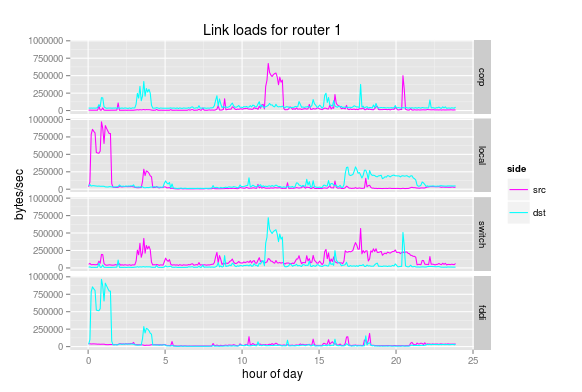
\includegraphics[scale=0.50]{./img/linkload_rout1.png}
\captionof{figure}{Link loads on different node of router 1's subnetwork, replicating Cao et al. figure 2.}
\endgroup

\textit{question 1.2} We replicate figure 4 of the paper with \texttt{1router\_allcount.dat}, of log variance against log mean in two time windows of 55 minutes. Linear fits are plotted for unfixed slope and slopes fixed at $c = 1$ and $c=2$. From the plot $c=2$ seems to give better regression results.

\begingroup
\centering
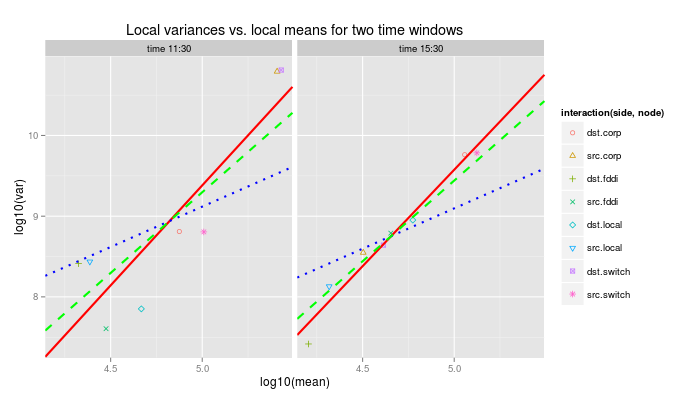
\includegraphics[scale=0.4]{./img/logvarlogmean.png}
\captionof{figure}{Local variances versus local means on log scale for the first data set. Linear regression in red, $c=1$ in dashed blue and $c=2$ in dashed green.}
\endgroup

Same figure is plotted for \texttt{2router\_linkcount.dat} on figure 3. In this dataset there are 8 different type of nodes, so 16 combinations of side (origin or destination) - node. Again $c=2$ seems to give better results than $c=1$.

\begingroup
\centering
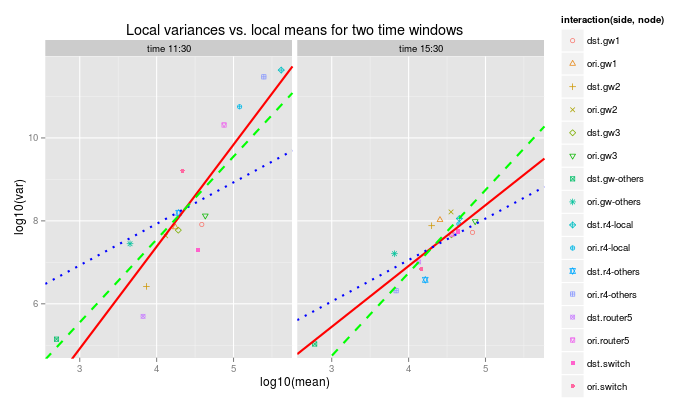
\includegraphics[scale=0.4]{./img/logvarlogmean2.png}
\captionof{figure}{Local variances versus local means on log scale for the second data set. Linear regression in red, $c=1$ in dashed blue and $c=2$ in dashed green.}
\endgroup

\vspace{.2 in}

\textit{question 1.3}

We model the $I$ unobserved OD counts $x_t$ at time $t$ as a vector of independent normal random variables
\begin{align*}
x_t \sim Normal(\lambda, \Sigma)
\end{align*}
with $\Sigma = \phi \* diag(\sigma^2(\lambda_1), ..., \sigma^2(\lambda_I))$, where $\sigma^2(\lambda) = \lambda^c$. And the observed link byte counts $y_t$ as
\begin{align*}
y_t = A \* x_t \sim Normal(A \* \lambda, A \* \Sigma A')
\end{align*}

We base inference on maximum likelihood on iid measurement of this distribution. There is no closed form solution to the likelihood maximization, so that an EM algorithm is implemented to find the parameter solution.\\

We do not assume a particular value for $c$, and our parameter is $\theta = \left(\lambda, \phi\right)$ ($16 + 1 = 17$ dimensional).\\

The EM conditional expectation function $Q$ is
\begin{align*}
Q(\theta, \theta^{(k)}) = E_q \left[ log\left(p(y, x | \theta) \right) \right]
\end{align*}
With $q = p(x | y, theta^{(k)})$, so that
\begin{align*}
Q(\theta, \theta^{(k)}) & = E \left[ log\left(p(Y, X | \theta)\right) | Y, \theta^{(k)} \right]\\
& = E \left[ log\left(p(X | \theta)\right) | Y, \theta^{(k)} \right]\\
& = E \left[ l(\theta|X) | Y, \theta^{(k)} \right]\\
\end{align*}
With $l(\theta|X)$ latent variable likelihood. We have
\begin{align*}
l(\theta | X) & = - \frac{T}{2} \* log|\Sigma| - \frac{1}{2	} \* \sum_{t=1}^{T} (x_t - \lambda)' \* \Sigma^{-1} \* (x_t - \lambda)\\
& = - \frac{T}{2} \* log|\Sigma| - \frac{1}{2} \* \sum_{t=1}^{T} x_t' \* \Sigma^{-1} \* x_t - \frac{1}{2} \* \sum_{t=1}^{T} x_t' \* \Sigma^{-1} \* \lambda - \frac{1}{2} \* \sum_{t=1}^{T}  \lambda' \* \Sigma^{-1} \* x_t - \frac{1}{2	} \* \sum_{t=1}^{T} \lambda' \* \Sigma^{-1} \* \lambda\\
\end{align*}
So that, taking expectation given $(Y, \theta^{(k)})$
\begin{align*}
Q(\theta, \theta^{(k)}) = & - \frac{T}{2} \* log|\Sigma| - \frac{1}{2} \* \sum_{t=1}^{T} \left( tr(\Sigma^{-1} \* var(x_t| Y, \theta^{(k)})) + E(x_t' | Y, \theta^{(k)}) \* \Sigma^{-1} \* E(x_t | Y, \theta^{(k)}) \right) \\
& - \frac{1}{2} \* \sum_{t=1}^{T} E(x_t' | Y, \theta^{(k)}) \* \Sigma^{-1} \* \lambda - \frac{1}{2} \* \sum_{t=1}^{T}  \lambda' \* \Sigma^{-1} \* E(x_t | Y, \theta^{(k)}) - \frac{1}{2	} \* \sum_{t=1}^{T} \lambda' \* \Sigma^{-1} \* \lambda\\
\end{align*}
Using the variance formula for a quadratic form to compute the second term, $E(\epsilon' \Lambda \epsilon) = tr(\Lambda \epsilon) + \mu' \* \Lambda \mu$. As $x_t$ is only dependent on $y_t$, the conditional expectation function simplifies to
\begin{align*}
Q(\theta, \theta^{(k)}) = & - \frac{T}{2} \* \left(log|\Sigma| + tr(\Sigma^{-1} \* R^{(k)}) \right) - \frac{1}{2} \* \sum_{t=1}^{T} (m_t^{(k)} - \lambda)' \* \Sigma^{-1} \* (m_t^{(k)} - \lambda) \\
\end{align*}
Where we have conditional mean and variance of $x_t$
\begin{align*}
m_t^{(k)} & = E\left(x_t | y_t, \theta^{(k)}\right)\\
& = \lambda^{(k)} + \Sigma^{(k)} A' (A \Sigma^{(k)} A' )^{-1} \left(y_t - A \lambda^{(k)}\right)\\
R^{(k)} & = var\left(x_t | y_t, \theta^{(k)}\right)\\
& = \Sigma^{(k)} - \Sigma^{(k)} A' (A \Sigma^{(k)} A' )^{-1} A \Sigma^{(k)}
\end{align*}
Those expression are derived by considering the multivariate normal vector $(x_t, y_t)$, and apply formulas for projected multivariate normals given that $cov(x_t, y_t) = cov(x_t, A x_t) = A \* \Sigma^{(k)}$ and $cov(y_t, y_t) = A \* \Sigma^{(k)} \* A'$ given $\theta^{(k)}$.\\

Expanding the expression of $Q$, we have
\begin{align*}
Q(\theta, \theta^{(k)}) = & - \frac{T}{2} \sum_{i = 1}^I c \* log(\lambda_i) - \frac{T}{2} \sum_{i = 1}^{I} \frac{r_{i i}^{(k)}}{\phi \* \lambda_i^{c}} - \frac{1}{2} \* \sum_{t=1}^{T} \sum_{i=1}^I \frac{(m_{t, i}^{(k)})^2}{\phi \* \lambda_i^c}\\
& + \sum_{t=1}^T \sum_{i=1}^I \frac{\lambda_i \* m_{t, i}^{(k)}}{\phi \* \lambda_i^c} - \frac{1}{2} \* \sum_{t=1}^T \sum_{i=1}^I \frac{\lambda_i^2}{\phi \* \lambda_i^c}
\end{align*}

So that taking $\frac{\partial Q}{\partial \theta}$ gives us the system of equations (first I ones due to $\lambda$, last one to $\phi$)
\begin{eqnarray}
c \phi \lambda_i^{c} + (2 - c) \lambda_i^2 - 2 ( 1 -c) \lambda_i b_i^{(k)} - c a_i^{(k)} = 0 &  \quad i = 1...I \\
\sum_{i = 1}^I \lambda_i^{-c + 1} ( \lambda_i - b_i^{(k)} )  = 0 &
\end{eqnarray}
Where we have defined
\begin{align*}
a_i^{(k)} & = r_{i i}^{(k)} + \frac{1}{T} \* \sum_{t=1}^T (m_{t, i}^{(k)})^2\\
b_i^{(k)} & = \frac{1}{T} \* \sum_{t=1}^T m_{t, i}^{(k)}
\end{align*}


We hence derive the steps of the EM algorithm for our iid model.\\

\vspace{.2 in}
\begin{algorithm}[H]
 \KwData{Observed link loads Y.}
 \KwResult{MLE of parameter $\theta$.}
 initialization: $\theta = \theta_0$ positive parameter.\\
 \While{$|Q(\theta^{(k + 1}, \theta^{(k)}) - Q(\theta^{(k)}, \theta^{(k - 1)})| > \epsilon$}{
  - Update step: k = k + 1\\
  - E-step: Compute $m_t^{(k)}, R^{(k)}, a_i^{(k)}, b_i^{(k)}$.\\
  - M-step
  \eIf{c = 1 or c = 2}{
   1. Solve (1) for $\lambda$ analytically given $\phi$ (positive solution).\\
   2. Solve for $\phi$ using fractional steps Newton-Raphson or constrained \texttt{optim} optimization (ensures $\phi$ positive).
   }{
   Update $\theta$ using constrained \texttt{optim} optimization (ensures parameters positive).
  }
 }
 \caption{EM algorithm for iid model}
\end{algorithm}
\vspace{.2 in}

\textit{question 1.4} We fix the variance and window frame paramters to be $c = 2$ (most appropriate according to exploratory data analysis), $w=11$. The MLE equations (1) then becomes
\begin{align*}
\phi \lambda_i^{2} + \lambda_i b_i^{(k)} - a_i^{(k)} = 0 &  \quad i = 1...I \\
\end{align*}
Which gives us a positive solution (the biggest of the two roots of the equation) for $\lambda_i$ given $\phi$
\begin{align*}
\lambda^{(k + 1)}_i = \frac{\sqrt{(b_i^{(k)})^2 + 4 \phi^{(k)} a_i^{(k)}} - b_i^{(k)}}{2 \phi^{(k)}}
\end{align*}
Setting $\lambda$ to those values, we have $f_i(\theta) = 0$ for $i = 1..I$ where $f(\theta)$ is the left hand-side of equations (1) and (2), so that the one-step Newton-Raphson algorithm
\begin{align*}
\theta^{(k + 1)} = \theta^{(k)} - \left[ F ( \theta^{(k)} ) \right]^{-1} \* f(\theta^{(k)})
\end{align*}
Reduces to
\begin{align*}
\phi^{(k + 1)} = \phi^{(k)} - \left(\left[ F ( \theta^{(k)} ) \right]^{-1}\right)_{I + 1, I + 1} \* f_{I + 1}(\theta^{(k)})
\end{align*}
With
\begin{align*}
f_{I + 1}(\theta^{(k)}) = \sum_{i = 1}^I \frac{\lambda_i - b_i^{(k)}}{\lambda_i}\\
\end{align*}
And the Jacobian $F ( \theta^{(k)})$ defined by
\begin{align*}
& \frac{\partial f_i}{\partial \lambda_j} = \delta_{i j} \left( \frac{4 \phi}{\lambda_i} + 2 b_i^{(k)} \right)\\
& \frac{\partial f_{I + 1}}{\partial \lambda_j} = \frac{b_j^{(k)}}{\lambda_j}\\
& \frac{\partial f_i}{\partial \phi} = 2 \lambda_i^2\\
& \frac{\partial f_{I + 1}}{\partial \phi} = 0\\
\end{align*}
To solve the M-step of our EM algorithm, we adopt an iterative fractional Newton-Raphson method, by dividing the step in the former udpate of $\phi$ by bigger and bigger integer if the update is negative. However this approach failed to converge fast enough (steps are too small), and we falled back on an \texttt{optim} optimization method.
\vspace{.2 in}
We extend the basic iid model to a local idd model, by setting time moving windows in which observations are treated iid.
\begin{align*}
y_{t - h}, ..., y_{t + h} \sim Normal(A \lambda_t, A \Sigma_t A' )
\end{align*}
With $\Sigma_t = \phi_t diag(\lambda_t^2)$. On each of those windowed data set, the MLE parameter $\theta_t$ is fitted using the previously derived iid model EM.

\vspace{.2 in}
\textit{question 1.5} We derive the EM algorithm for the refined model of the paper's fourth section. This refined model adds smoothing to the estimates by considering the parameters as following hidden markov model, resulting in an algorithm similar to the Kalman Filter.\\

$\eta_t = (log(\lambda_t), log(\phi_t))$ is modeled as a random walk state
\begin{align*}
\eta_t = \eta_{t - 1} + v_t
\end{align*} 
With $v_t \sim Normal(0, V)$, and V fixed variance matrix. We denote all the current information until time $t + h$ by $\tilde{Y_{t}} = (y_1, ..., y_{t + h})$, and the window data set at time t $Y_t$. The goal of our EM algorithm is to find the MAP estimator, ie. the mode of the posterior distribution $p(\eta_t | \tilde{Y_{t}})$.\\

We actually have
\begin{align*}
p(\eta_t | \tilde{Y}_{t}) = p(\eta_t | \tilde{Y}_{t - 1}, Y_t) \propto p(\eta_t | \tilde{Y}_{t - 1}) p(Y_t | \eta_t)
\end{align*}
Using Baye's rule.


%----------------------------------------------------------------------------------------

%\end{multicols}

\end{document}
